
\section{Prerequisites}

As I'm working through Spivak, I'm regularly discovering there is a
ton of high school math I've forgotten (or simply never learned). The
purpose of this chapter is to relearn the necessary prerequisites as
quickly as possible.

\vs

I pull in prerequisites ``lazily''. There is no predefined set of
topics; nothing that ``should (or shouldn't) be a part of
precalculus''. When I need to know something to get through Spivak's
chapter but don't already know it, it goes here.

\vs

A lot of material I'm pulling from ``Paul's Online Notes'' excellent
\href{https://tutorial.math.lamar.edu/Extras/AlgebraTrigReview/AlgebraTrig.aspx}{Algebra
  Trig Review}. He definitely nails the topic list-- the stuff his
calculus students forgot (or never learned) lines up really well with
what I need.

\subsection{Inequalities}
Consider an inequality $0<|x-a|<\delta$. This will come up a lot soon. What
does this inequality mean? The intuitive reading is that the
difference between $x$ and $a$ is between $0$ and $\delta$. But it's a
little subtle, so let's look at it carefully. There are actually two
inequalities here: $0<|x-a|$ and $|x-a|<\delta$. We should consider each
separately.

\vs

The left side, $0<|x-a|$ is equivalent to $|x-a|>0$. But $|x-a|$ is an
absolute value, it's \textbf{always} true that $|x-a|\geq 0$. So this
part of the inequality says $x-a\neq 0$, or $x\neq a$. I don't know why
mathematicians say $0<|x-a|$ instead of $x\neq a$, probably because
confusing you brings them pleasure.

\vs

The right side is $|x-a|<\delta$. Intuitively this says that the difference
between $x$ and $a$ should be less than $\delta$. Put differently, $x$
should be within $\delta$ of $a$. Algebraically we can write it as two
cases:
\begin{enumerate}
\item $x-a<\delta$
\item $-(x-a)<\delta$
\end{enumerate}
A little basic manipulation, and we can rewrite this as $a-\delta<x<a+\delta$.

\subsubsection*{Bounding}
We will often need to make an inequality of the following form work out:

\[|n||m|<\epsilon\]

Here $\epsilon$ is given to us, we have complete control over the upper bound
of $|n|$, and $|m|$ can take on values outside our direct control.
Obviously we can't make the inequality work without knowing
\textit{something} about $|m|$, so we'll try to find a bound for it in
terms of other fixed values, or values we control.

\vs

For example, suppose we've discovered there is a fixed value $a$, and
that $|m|<3|a|+4$. Given that we control $|n|$, how do we bound it in
terms of $\epsilon$ and $|a|$ in such a way that the inequality
$|n||m|<\epsilon$ holds?

\vs

Since we control $|n|$ and $(3|a|+4)$ is fixed, we can find $|n|$
small enough so that $|n|(3|a|+4)<\epsilon$ holds. Then certainly any
inequality whose left side is smaller, e.g. $|n|(3|a|+3)<\epsilon$, will also
hold. And since $|m|$ is always smaller than $3|a|+4$, it follows
$|n||m|<\epsilon$ will hold as well.

\vs

All we have left to do is find a bound for $|n|$ such that
$|n|(3|a|+4)<\epsilon$ holds, which is of course easy:

\[|n|<\frac{\epsilon}{3|a|+4}\]

Having bound $|n|$ in this way, we can verify that
$|n|(3|a|+4)<\epsilon$ holds by multiplying both sides of the above
inequality by $3|a|+4$.

\subsection{Trigonometry}

Let $P$ be a point on a unit circle $x^2+y^2=1$. Let $\theta$ be the length
of the arc from $(1,0)$ to $P$, measured counterclockwise along the
circle. Then the coordinates of $P$ are
$(\cos\theta,\sin\theta)$.\footnote{The order is easy to remember-- it's
  alphabetical.}

\begin{figure}[htbp]
  \centering
  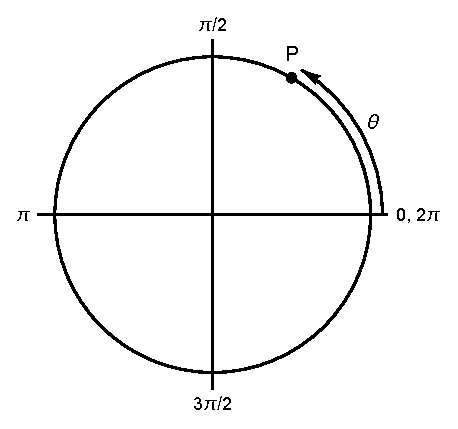
\includegraphics[width=0.5\textwidth]{eps/prereqs/trigtldr.eps}
\end{figure}

The measure of angles by the length of the arc is in units called
\textit{radians}. Recall the circumference of a circle is $C=2\pi r$,
and so the circumference of a unit circle is $2\pi$. Thus $\pi$ represents
a $180^\circ$ angle. Some common angles in radians are
$2\pi, \pi,\frac{\pi}{2}, \frac{\pi}{3}, \frac{\pi}{4}, \frac{\pi}{6}$, and
$\frac{3\pi}{2}$. To convert these to degrees simply replace $\pi$ with
$180$, and compute the fraction.

\vs

It should be self-evident that adding $2\pi$ to an angle results in the
angle itself; and that adding $\frac{\pi}{2}$ to an angle shifts it by
$90^{\circ}$. Further:
\[(\cos 0,\sin 0)=(1,0)\ \ \ \ \ \text{and}\ \ \ \ \ (\cos \frac{\pi}{2},\sin \frac{\pi}{2})=(0,1)\]

\subsubsection*{Plotting}
It is not too difficult to plot trigonometric functions. Consider some
properties of cosine we've already seen (or can easily deduce):
$\cos 0=1$, $\cos \frac{\pi}{2}=0$, $\cos \pi=-1$. We've also seen that
$\cos{(x+2\pi)}=\cos x$. The $x$-axis below covers $[-3\pi, 3\pi]$ (i.e. a
total length of $6\pi$). Since cosine repeats every $2\pi$, we should
expect the graph to repeat thrice. And this is exactly what we see.
\begin{figure}[htbp]
  \centering
  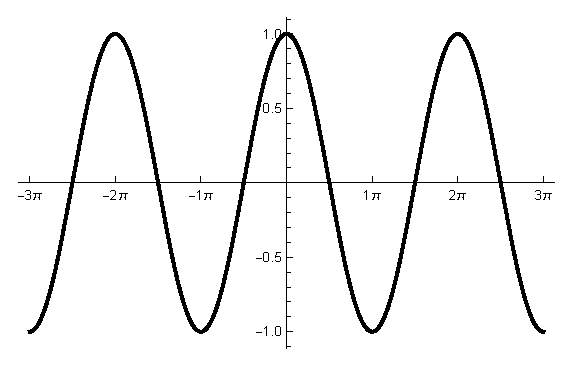
\includegraphics[width=.75\textwidth]{eps/prereqs/cosine.eps}
\end{figure}

We can easily increase the frequency by plotting $y=\cos cx$. Here we
double the frequency with $c=2$:
\begin{figure}[htbp]
  \centering
  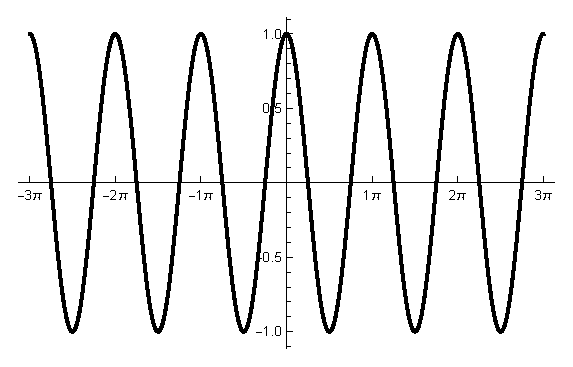
\includegraphics[width=.75\textwidth]{eps/prereqs/cosine2x.eps}
\end{figure}

\subsection{Limits}

Here I only present a hand-wavy definition of limits and use it to
explain the mechanics of computing limits of functions in practice. A
proper definition and proofs of the theorems that make the mechanics
work come in a later chapter.

\vs

\textbf{A hand-wavy definition:} a limit of $f(x)$ at $a$ is the value
$f(x)$ approaches close to (but not necessarily at) $a$.

\vs

\textbf{A slightly less hand-wavy definition:} let $f:\R\to\R$, let
$a\in\R$ be some number on the x-axis, and let $l\in\R$ be some number on
the y-axis. Then as $x$ gets closer to $a$, $f(x)$ gets closer to $l$.

\vs

The notation for this whole thing is

\[\lim_{x\to a} f(x)=l\]

So for example $\lim_{x\to5}x^2=25$ because the closer $x$ gets to
$5$, the closer $x^2$ gets to $25$ (we'll prove all this properly
soon). Now suppose you have some fancy pants function like this one:
\begin{equation}
\label{eq:1}
\lim_{x\to 0}\frac{1-\sqrt{x}}{1-x}
\end{equation}

If you plot it, it's easy to see that as $x$ approaches $0$, the whole
shebang approaches $1$. But how do you algebraically evaluate the
limit of this thing? Can you just plug $0$ into the equation? It seems
to work, but once we formally define limits, we'll have to prove
somehow that plugging $a=0$ into $x$ gives us the correct result.

\subsubsection*{Limits evaluation mechanics}

It turns out that it does in fact work because of a few theorems that
make practical evaluation of many limits easy. Here I'll state these
theorems as facts. Once I introduce the formal definition of limits in
a later chapter I'll properly prove them.

\begin{enumerate}
\item \textbf{Constants}. $\lim_{x\to a}c=c$, where $c\in\R$. In other
  words if the function is a constant, e.g. $f(x)=5$, then
  $\lim_{x\to a}f(x)=5$ for any $a$.
\item \textbf{Identity}. $\lim_{x\to a}x=a$. In other words if the
  function is an identity function $f(x)=x$, then
  $\lim_{x\to 6}f(x)=6$. Meaning we simply plug $a$ into $x$.
\item \textbf{Addition}\footnote{Spivak's book uses a slightly more
    verbose definition that assumes the limits of $f$ and $g$ exist
    near $a$, see p. 103}.
  $\lim_{x\to a}(f+g)(x)=\lim_{x\to a}f(x)+\lim_{x\to a}g(x)$. For example
  $\lim_{x\to a}(x+2)=\lim_{x\to a}x+\lim_{x\to a}2=a+2$.
\item \textbf{Multiplication}.
  $\lim_{x\to a}(f\cdot g)(x)=\lim_{x\to a}f(x)\cdot \lim_{x\to a}g(x)$. For example
  $\lim_{x\to a}2x=\lim_{x\to a}2\cdot \lim_{x\to a}x=2a$.
\item \textbf{Reciprocal}.
  $\lim_{x\to a}\left(\frac{1}{f}\right)(x)=\frac{1}{\lim_{x\to a}f(x)}$
  when the denominator isn't zero. For example
  $\lim_{x\to a}\frac{1}{x}=\frac{1}{\lim_{x\to a}x}=\frac{1}{a}$ for
  $a\neq0$.
\end{enumerate}

To come back to \ref{eq:1}, these theorems tells us that

\[\lim_{x\to 0}\frac{1-\sqrt{x}}{1-x}=\frac{\lim_{x\to 0}1-(\lim_{x\to 0}x)^{\frac{1}{2}}}{\lim_{x\to 0}1-\lim_{x\to 0}x}=\frac{1-0^{\frac{1}{2}}}{1-0}=1\]

\subsubsection*{Holes}

What happens if we try to take a limit as $x\to 1$ rather than $x\to 0$?

\[\lim_{x\to 1}\frac{1-\sqrt{x}}{1-x}\]

We can't use the same trick and plug in $1$ because we get a
nonsensical result $0/0$ as the function isn't defined at $0$. If we
plot it, we clearly see the limit approaches $1/2$ at $0$, but how do
we prove this algebraically? The answer is to do some trickery to find
a way to cancel out the inconvenient term (in this case $1-\sqrt{x}$)

\[\lim_{x\to 1}\frac{1-\sqrt{x}}{1-x}=\lim_{x\to 1}\frac{1-\sqrt{x}}{(1-\sqrt{x})(1+\sqrt{x})}=\lim_{x\to 1}\frac{1}{1+\sqrt{x}}=\frac{1}{2}\]

\vs

Why is it ok here to divide by $1-\sqrt{x}$? Good question! Recall
that the limit is defined \textit{close to} $a$ (or \textit{around}
$a$, or as $x$ \textit{approaches} $a$), but not \textbf{at} $a$. In
other words $f(a)$ need not even be defined (as is the case here).
This means that as we consider $1-\sqrt{x}$ at different values of $x$
as it approaches $a$, the limit never requires us to evaluate the
function at $x=a$. So we never have to consider $1-\sqrt{x}$ as $x=1$,
$1-\sqrt{x}$ never takes on the value of $0$, and it is safe to divide
it out.


%%% Local Variables:
%%% TeX-master: "notes"
%%% End:
